%generated tex file
\begin{figure}[h!]
    		\begin{center}
      			\includegraphics[width=0.3\linewidth,height=.7\paperheight,keepaspectratio]{retrogenerated_uml/exceptionwindow.png}
      			\caption{Diagramme de classe du package exceptionwindow}
    		\end{center}
  	\end{figure}
\begin{figure}[h!]
    		\begin{center}
      			\includegraphics[width=\linewidth,height=.7\paperheight,keepaspectratio]{retrogenerated_uml/citymapdetails.png}
      			\caption{Diagramme de classe du package citymapdetails}
    		\end{center}
  	\end{figure}
\begin{figure}[h!]
    		\begin{center}
      			\includegraphics[width=0.3\linewidth,height=.7\paperheight,keepaspectratio]{retrogenerated_uml/intersectioncard.png}
      			\caption{Diagramme de classe du package intersectioncard}
    		\end{center}
  	\end{figure}
\begin{figure}[h!]
    		\begin{center}
      			\includegraphics[width=0.3\linewidth,height=.7\paperheight,keepaspectratio]{retrogenerated_uml/informationarea.png}
      			\caption{Diagramme de classe du package informationarea}
    		\end{center}
  	\end{figure}
\begin{figure}[h!]
    		\begin{center}
      			\includegraphics[width=\linewidth,height=.7\paperheight,keepaspectratio]{retrogenerated_uml/mapscreen.png}
      			\caption{Diagramme de classe du package mapscreen}
    		\end{center}
  	\end{figure}
\begin{figure}[h!]
    		\begin{center}
      			\includegraphics[width=\linewidth,height=.7\paperheight,keepaspectratio]{retrogenerated_uml/components.png}
      			\caption{Diagramme de classe du package components}
    		\end{center}
  	\end{figure}
\begin{figure}[h!]
    		\begin{center}
      			\includegraphics[width=\linewidth,height=.7\paperheight,keepaspectratio]{retrogenerated_uml/events.png}
      			\caption{Diagramme de classe du package events}
    		\end{center}
  	\end{figure}
\begin{figure}[h!]
    		\begin{center}
      			\includegraphics[width=\linewidth,height=.7\paperheight,keepaspectratio]{retrogenerated_uml/timefield.png}
      			\caption{Diagramme de classe du package timefield}
    		\end{center}
  	\end{figure}
\begin{figure}[h!]
    		\begin{center}
      			\includegraphics[width=0.3\linewidth,height=.7\paperheight,keepaspectratio]{retrogenerated_uml/deliveryrequestdetails.png}
      			\caption{Diagramme de classe du package deliveryrequestdetails}
    		\end{center}
  	\end{figure}
\begin{figure}[h!]
    		\begin{center}
      			\includegraphics[width=\linewidth,height=.7\paperheight,keepaspectratio]{retrogenerated_uml/application.png}
      			\caption{Diagramme de classe du package application}
    		\end{center}
  	\end{figure}
\begin{figure}[h!]
    		\begin{center}
      			\includegraphics[width=\linewidth,height=.7\paperheight,keepaspectratio]{retrogenerated_uml/waypointcard.png}
      			\caption{Diagramme de classe du package waypointcard}
    		\end{center}
  	\end{figure}
\begin{figure}[h!]
    		\begin{center}
      			\includegraphics[width=\linewidth,height=.7\paperheight,keepaspectratio]{retrogenerated_uml/planningdetails.png}
      			\caption{Diagramme de classe du package planningdetails}
    		\end{center}
  	\end{figure}
\begin{figure}[h!]
    		\begin{center}
      			\includegraphics[width=\linewidth,height=.7\paperheight,keepaspectratio]{retrogenerated_uml/mapcanvas.png}
      			\caption{Diagramme de classe du package mapcanvas}
    		\end{center}
  	\end{figure}
\begin{figure}[h!]
    		\begin{center}
      			\includegraphics[width=0.3\linewidth,height=.7\paperheight,keepaspectratio]{retrogenerated_uml/main.png}
      			\caption{Diagramme de classe du package main}
    		\end{center}
  	\end{figure}
\begin{figure}[h!]
    		\begin{center}
      			\includegraphics[width=\linewidth,height=.7\paperheight,keepaspectratio]{retrogenerated_uml/tsp.png}
      			\caption{Diagramme de classe du package tsp}
    		\end{center}
  	\end{figure}
\begin{figure}[h!]
    		\begin{center}
      			\includegraphics[width=\linewidth,height=.7\paperheight,keepaspectratio]{retrogenerated_uml/command.png}
      			\caption{Diagramme de classe du package command}
    		\end{center}
  	\end{figure}
\begin{figure}[h!]
    		\begin{center}
      			\includegraphics[width=\linewidth,height=.7\paperheight,keepaspectratio]{retrogenerated_uml/map.png}
      			\caption{Diagramme de classe du package map}
    		\end{center}
  	\end{figure}
\begin{figure}[h!]
    		\begin{center}
      			\includegraphics[width=\linewidth,height=.7\paperheight,keepaspectratio]{retrogenerated_uml/xml.png}
      			\caption{Diagramme de classe du package xml}
    		\end{center}
  	\end{figure}
\begin{figure}[h!]
    		\begin{center}
      			\includegraphics[width=\linewidth,height=.7\paperheight,keepaspectratio]{retrogenerated_uml/exception.png}
      			\caption{Diagramme de classe du package exception}
    		\end{center}
  	\end{figure}
\begin{figure}[h!]
    		\begin{center}
      			\includegraphics[width=0.3\linewidth,height=.7\paperheight,keepaspectratio]{retrogenerated_uml/tools.png}
      			\caption{Diagramme de classe du package tools}
    		\end{center}
  	\end{figure}
\begin{figure}[h!]
    		\begin{center}
      			\includegraphics[width=0.3\linewidth,height=.7\paperheight,keepaspectratio]{retrogenerated_uml/pdf.png}
      			\caption{Diagramme de classe du package pdf}
    		\end{center}
  	\end{figure}
\begin{figure}[h!]
    		\begin{center}
      			\includegraphics[width=\linewidth,height=.7\paperheight,keepaspectratio]{retrogenerated_uml/services.png}
      			\caption{Diagramme de classe du package services}
    		\end{center}
  	\end{figure}
\begin{figure}[h!]
    		\begin{center}
      			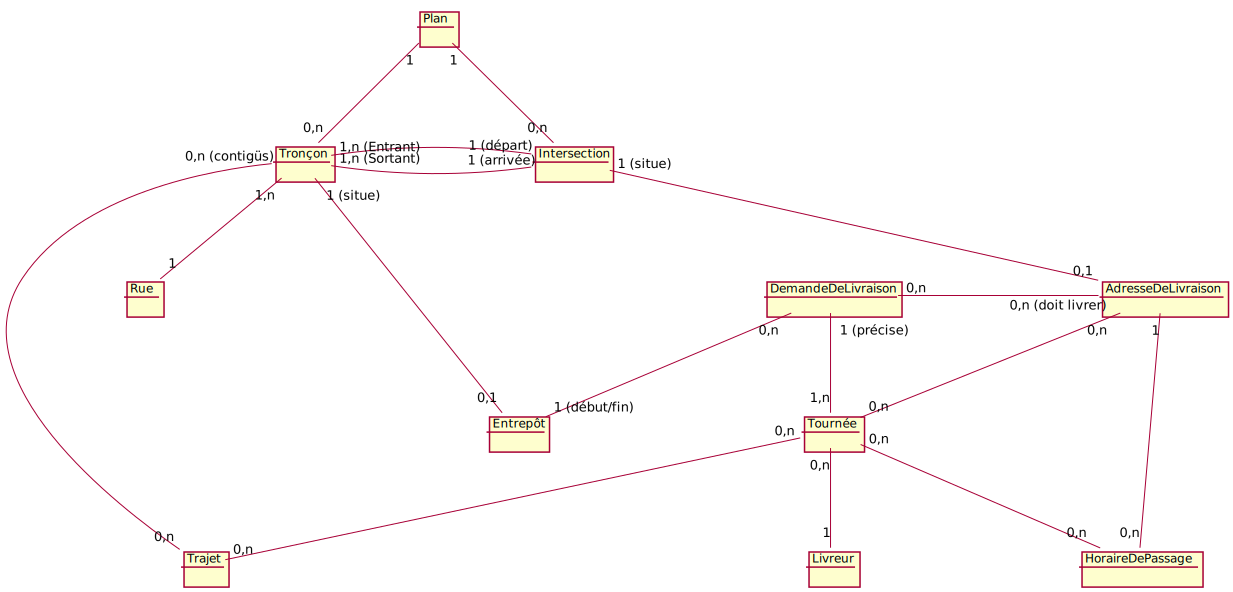
\includegraphics[width=\linewidth,height=.7\paperheight,keepaspectratio]{retrogenerated_uml/model.png}
      			\caption{Diagramme de classe du package model}
    		\end{center}
  	\end{figure}
\begin{figure}[h!]
    		\begin{center}
      			\includegraphics[width=\linewidth,height=.7\paperheight,keepaspectratio]{retrogenerated_uml/java.png}
      			\caption{Diagramme de classe du package java}
    		\end{center}
  	\end{figure}
